% results_section.tex: GENERATED, do not edit.
% Built by scripts/paper/build_section.jl on 2026-06-11 14:39
% from section_source.tex + values.tex; sweep 2026-06-07_f424438; repo commit 1a931f7.
% Every number was computed from the saved sweep data by scripts/paper/stats.jl.

\section{Results}

All results in this section are computed from a single parameter sweep of the
simulated market, run both without and with capture. In the baseline regime,
$N=1{,}000$ agents interact for $T=200$ periods with matching-function parameters
$\rho=0.5$ and $\delta=0.5$, turnover $\eta=0.02$, reservation threshold $f_r=0.6$,
and initial network degree $k_G=6$; the first 30 periods of each run are treated as
burn-in. Around this baseline we vary one parameter at a time
($\rho\in\{0,0.3,0.5,0.7,1\}$, $\eta\in\{0.01,0.02,0.03\}$,
$N\in\{500,1{,}000,1{,}500\}$, $f_r\in\{0.4,0.6,0.9,1.2\}$, $\delta\in\{0,0.75\}$,
$k_G\in\{4,12\}$, and, under capture only, the broker's capture accuracy gate
$\kappa_{\max}\in\{0.4,0.5,0.65\}$) and additionally sweep seven two-parameter
grids: the six pairwise combinations of $\{\rho,\eta,N,f_r\}$ and the
$\rho\times\delta$ grid (on the grids, $\rho$ takes the three levels $\{0,0.5,1\}$
and $\delta$ the levels $\{0,0.5,0.75\}$; the remaining axes reuse their
one-at-a-time levels). The design comprises 91 regimes without capture and
94 with capture, each simulated under five independent seeds
(925 runs in total); the same seeds are reused across regimes, so capture
and no-capture counterparts can be compared pairwise. Reported statistics are
ensemble means over seeds, summarized by time averages over fixed windows within a
run: late means over the final 20 periods ($t\in[181,200]$), used for all reported
levels unless noted otherwise, and early means over $t\in[50,70]$, which quantify
within-run drift. Full parameter values are given in Appendix~A~\S10, and every
statistic and figure is reproducible from the saved sweep.

\subsection{The broker primarily provides assessment, not access}

Across the simulations, the broker is the dominant channel in the market.
Principals route most demand to the broker rather than to self-search: the
outsourcing rate, the share of match demand sent to the broker, is
0.93 at the no-capture baseline (late mean, up from an early mean
of 0.81), and it stays high across the no-capture regimes (late
means of 0.73 to 0.98). Principals prefer the broker because
its matches are better. The realized value of broker-channel matches exceeds that
of self-search matches in 90 of 91 no-capture regimes, with
an output gap (broker minus self) averaging $+0.42$ across regimes
(late means). This is the model's rendering of why relational work gets
outsourced: the broker constructs better matches than clients do on their own.

What allows the broker to construct better matches is an advantage in assessment,
not access. The access fraction, the share of brokered placements between two
agents with no pre-existing tie, is low, with a late mean of
0.16 across no-capture regimes (down from
0.22 early), and it declines over time within the run in
91 of 91 regimes. Most brokered matches connect
principals who already knew each other; the broker's contribution is to identify
which of them pair well, not to provide reach (Fig.~\ref{fig:position}).

\begin{figure}[t]
\centering
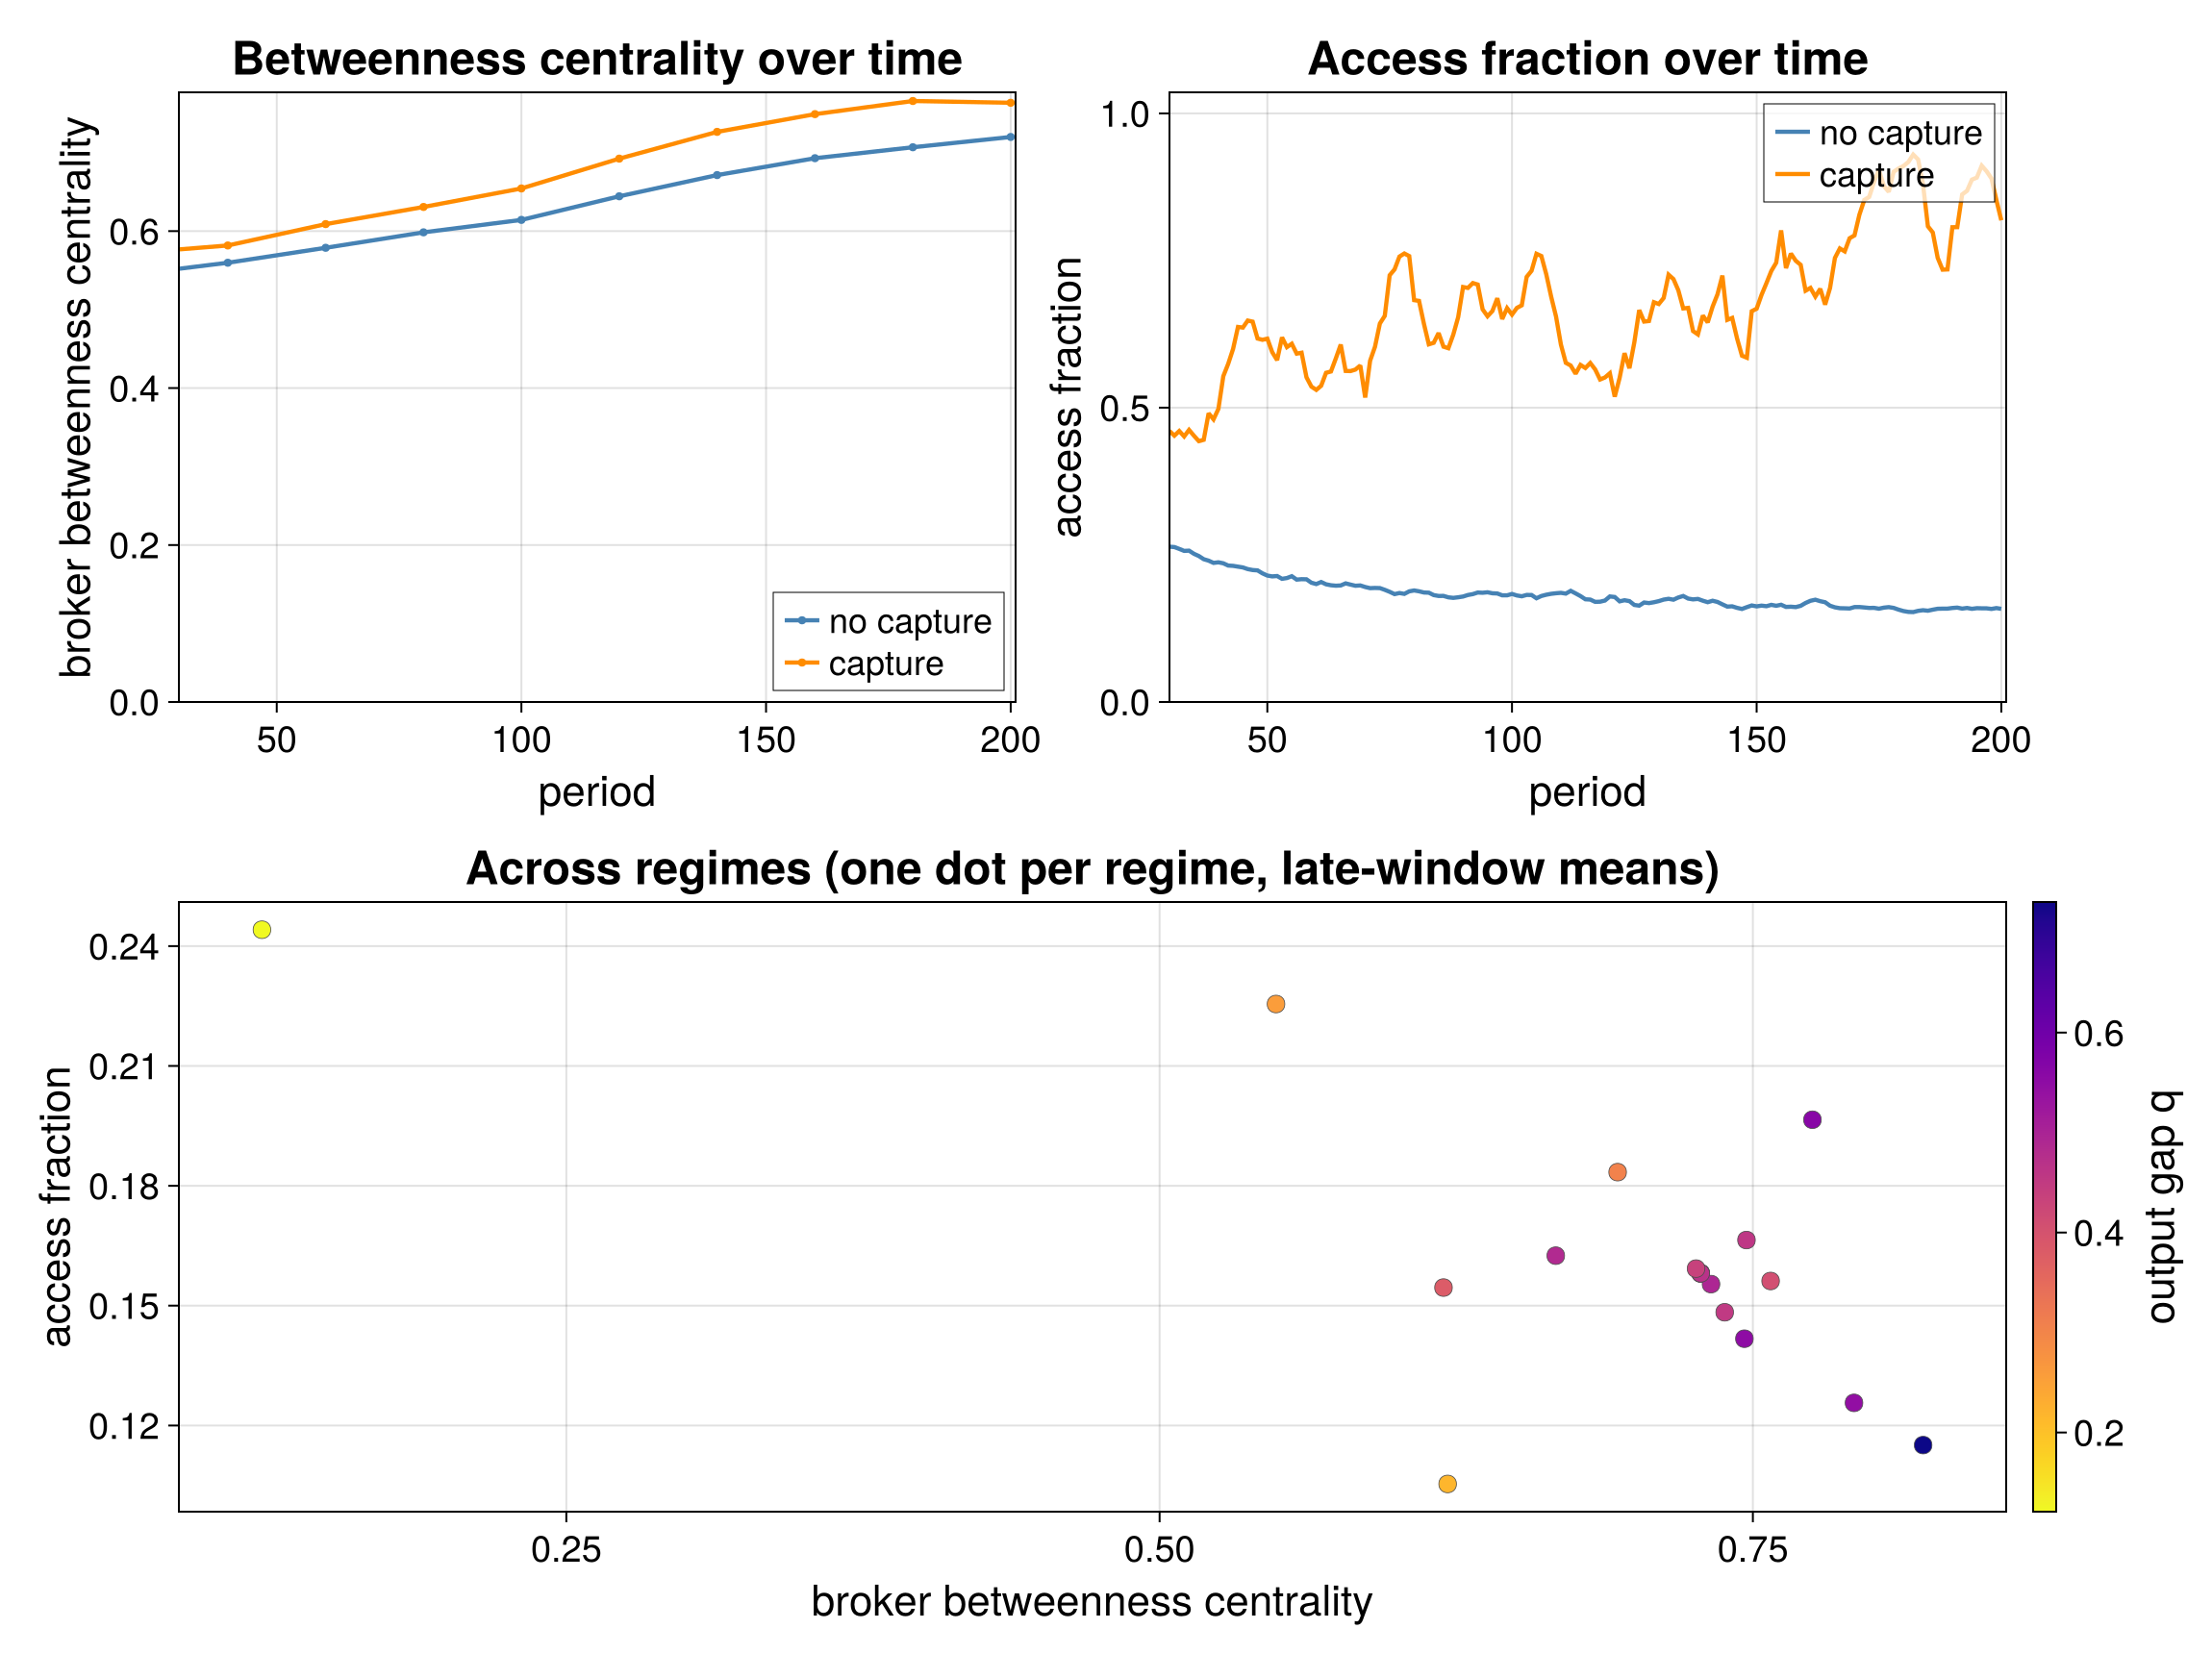
\includegraphics[width=0.92\linewidth]{figs/fig1_position_work.png}
\caption{Broker betweenness and access fraction. Top row: ensemble means over time
at the baseline regime pair (no capture, dashed; capture, solid), as 5-observation
rolling means; betweenness is measured every 20 periods. Bottom: late means across
the one-at-a-time no-capture regimes, one dot per regime, colored by the effective
rank $r_{90}$ of the matching function. Axes start at $t=30$ (end of burn-in).}
\label{fig:position}
\end{figure}

The broker's assessment advantage lies in better ranking, not in precise
valuation. On a held-out sample of random partners (Appendix~A~\S8), the broker
orders prospective pairings well (rank correlation of 0.89 with
the true ordering at the no-capture baseline, late mean, and
0.91 to 0.95 across the four easiest, $\delta=0$
regimes) but predicts output levels poorly (holdout $R^2$ of 0.65
at baseline, and negative on the hardest complementarity problems). Principals are
weak on both, with a holdout rank correlation of 0.51 and a
holdout $R^2$ of $-2.63$ (baseline, late means). Ranking is
what matchmaking requires, so what the broker's services rely on is a good
ordering of candidate pairings, more than an accurate appraisal of their absolute
worth.

Within the model, the broker acts not as an appraiser of general quality, but as a
matchmaker who knows which parties suit each other. Its value comes from the
ranking of complementarities, and it holds even where clients can reach
counterparties directly.

\subsection{How the matching problem shapes the broker's advantages}
\label{sec:matching-shapes}

Recall that $\rho$ sets the direction of the matching problem, from pure general
quality to pure complementarity, and that the gain $\delta$ sets its difficulty
through the effective rank of the output (see model description above).
Interestingly, across regimes, the broker's structural position tracks $\rho$
while its prediction edge tracks $\delta$, and the two need not move together.

The structural measures vary with $\rho$ and are nearly flat in $\delta$. Broker
betweenness, the share of shortest paths between agents that run through the
broker, is higher where matching is more complementarity-driven
(0.82 at $\rho=0$ against 0.12 at $\rho=1$; late means along the
one-at-a-time sweep, $\delta=0.5$), while at fixed $\rho=0.5$ it moves little with
the gain (0.69, 0.73, 0.75 at
$\delta=0,0.5,0.75$). The access fraction moves the opposite way
(0.12 against 0.24). Under complementarity ($\rho=0$), the
broker is more central but, in practice, bridges less: a larger share of its
matches re-pair agents already tied to each other.

Meanwhile, the prediction measures vary with $\delta$. Ordering is what the broker
needs, and its rank correlation with realized output stays high across regimes
(0.91 to 0.95 on the simplest problems,
0.89 at baseline, falling to 0.67 at
$\rho=0$, $\delta=0.75$; Fig.~\ref{fig:ranklines}), well above the agents'
throughout (0.51 at baseline). Performance at predicting the
output behaves differently: the broker's holdout $R^2$ at $\rho=0$ is
$+0.85$ when the output is simple but strongly negative when it is
complex ($-2.43$ at $\delta=0.5$ and $-3.89$ at
$\delta=0.75$, in the $\rho\times\delta$ grid, late means), worse than predicting
the average and, on the hardest complementarity problems, worse than the agents'
own (an $R^2$ gap of $-0.94$ at $\rho=0$, $\delta=0.75$), despite
the broker seeing both sides of every match and pooling across the market. Ranking
which match is better thus withstands difficulty far better than predicting how
good it will be, and the broker's ordering edge, though it narrows on the hardest
complementarity problems, is what persists.

\begin{figure}[t]
\centering
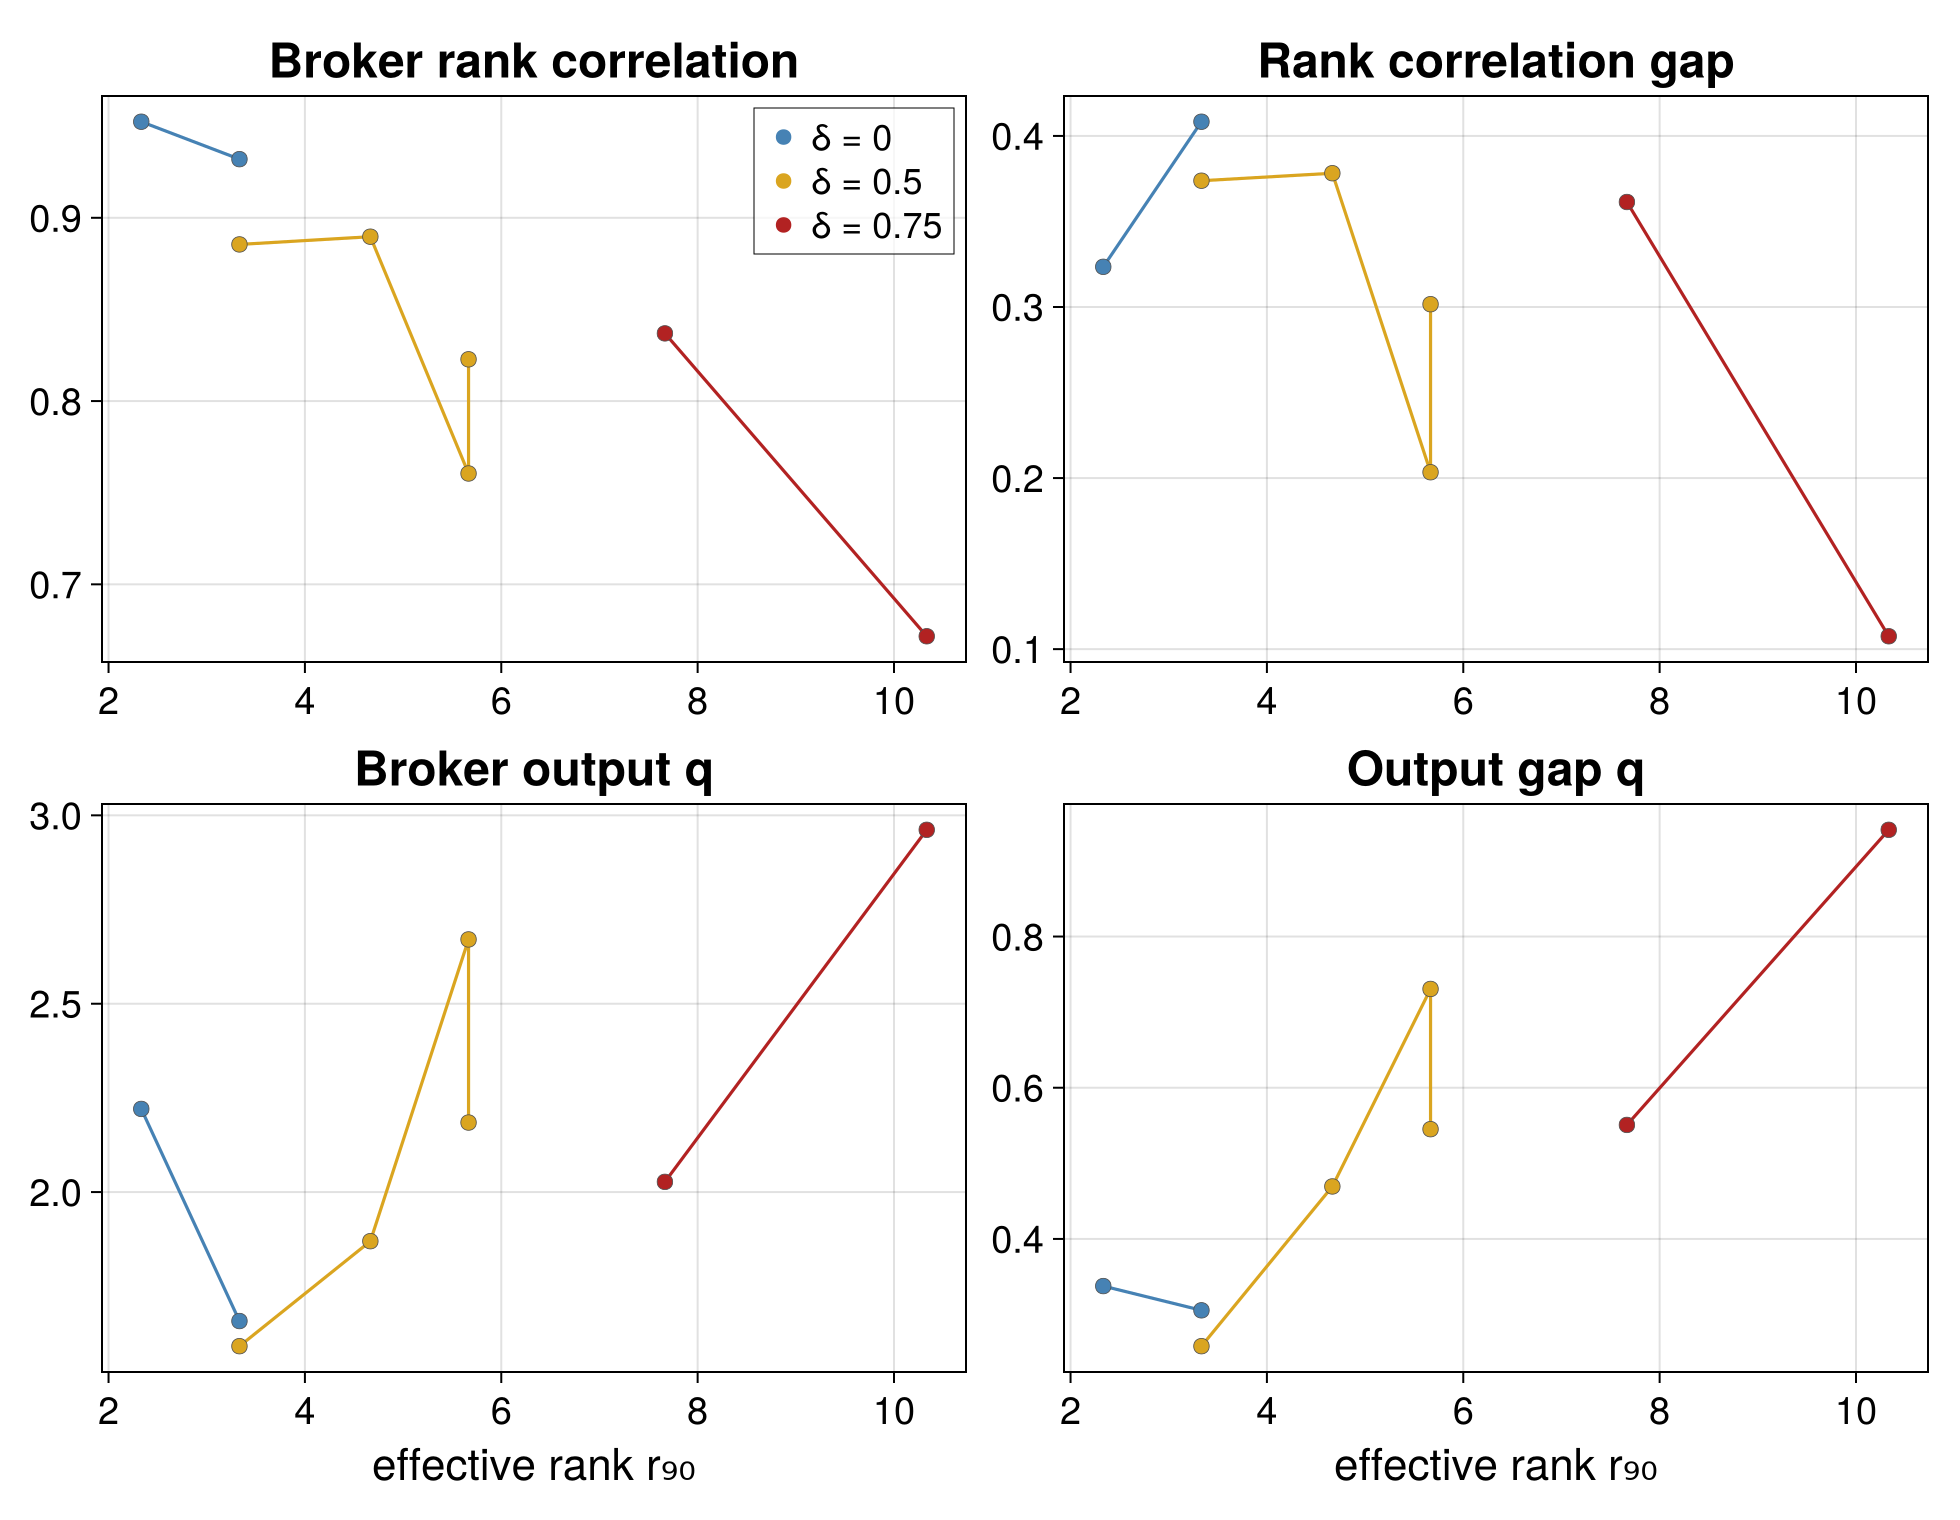
\includegraphics[width=0.78\linewidth]{figs/fig2_rank_lines.png}
\caption{Late means of four outcomes against the effective rank $r_{90}$ of the
matching function, across the $\rho\times\delta$ grid ($\rho=1$ omitted) plus the
one-at-a-time $\rho$ regimes; one line per gain $\delta$, no capture.}
\label{fig:ranklines}
\end{figure}

Realized match quality follows neither measure cleanly: the broker still produces
better matches than self-search wherever matching is relational, most of all where
it is also complex (the output gap is $+0.73$ at $\rho=0$, $\delta=0.5$,
against $+0.12$ at $\rho=1$; late means; Fig.~\ref{fig:grid}),
consistent with the idea that the broker matters most where match value turns on
complementarity. One pattern is unexplained, however. The broker's realized output
advantage is largest exactly where its ranking advantage over agents is smallest,
in the hard complementarity regimes: at $\rho=0$ the rank-correlation gap is
0.32 at $\delta=0$ and 0.11 at $\delta=0.75$ (grid,
late means). Why this is remains an open question.

\begin{figure}[t]
\centering
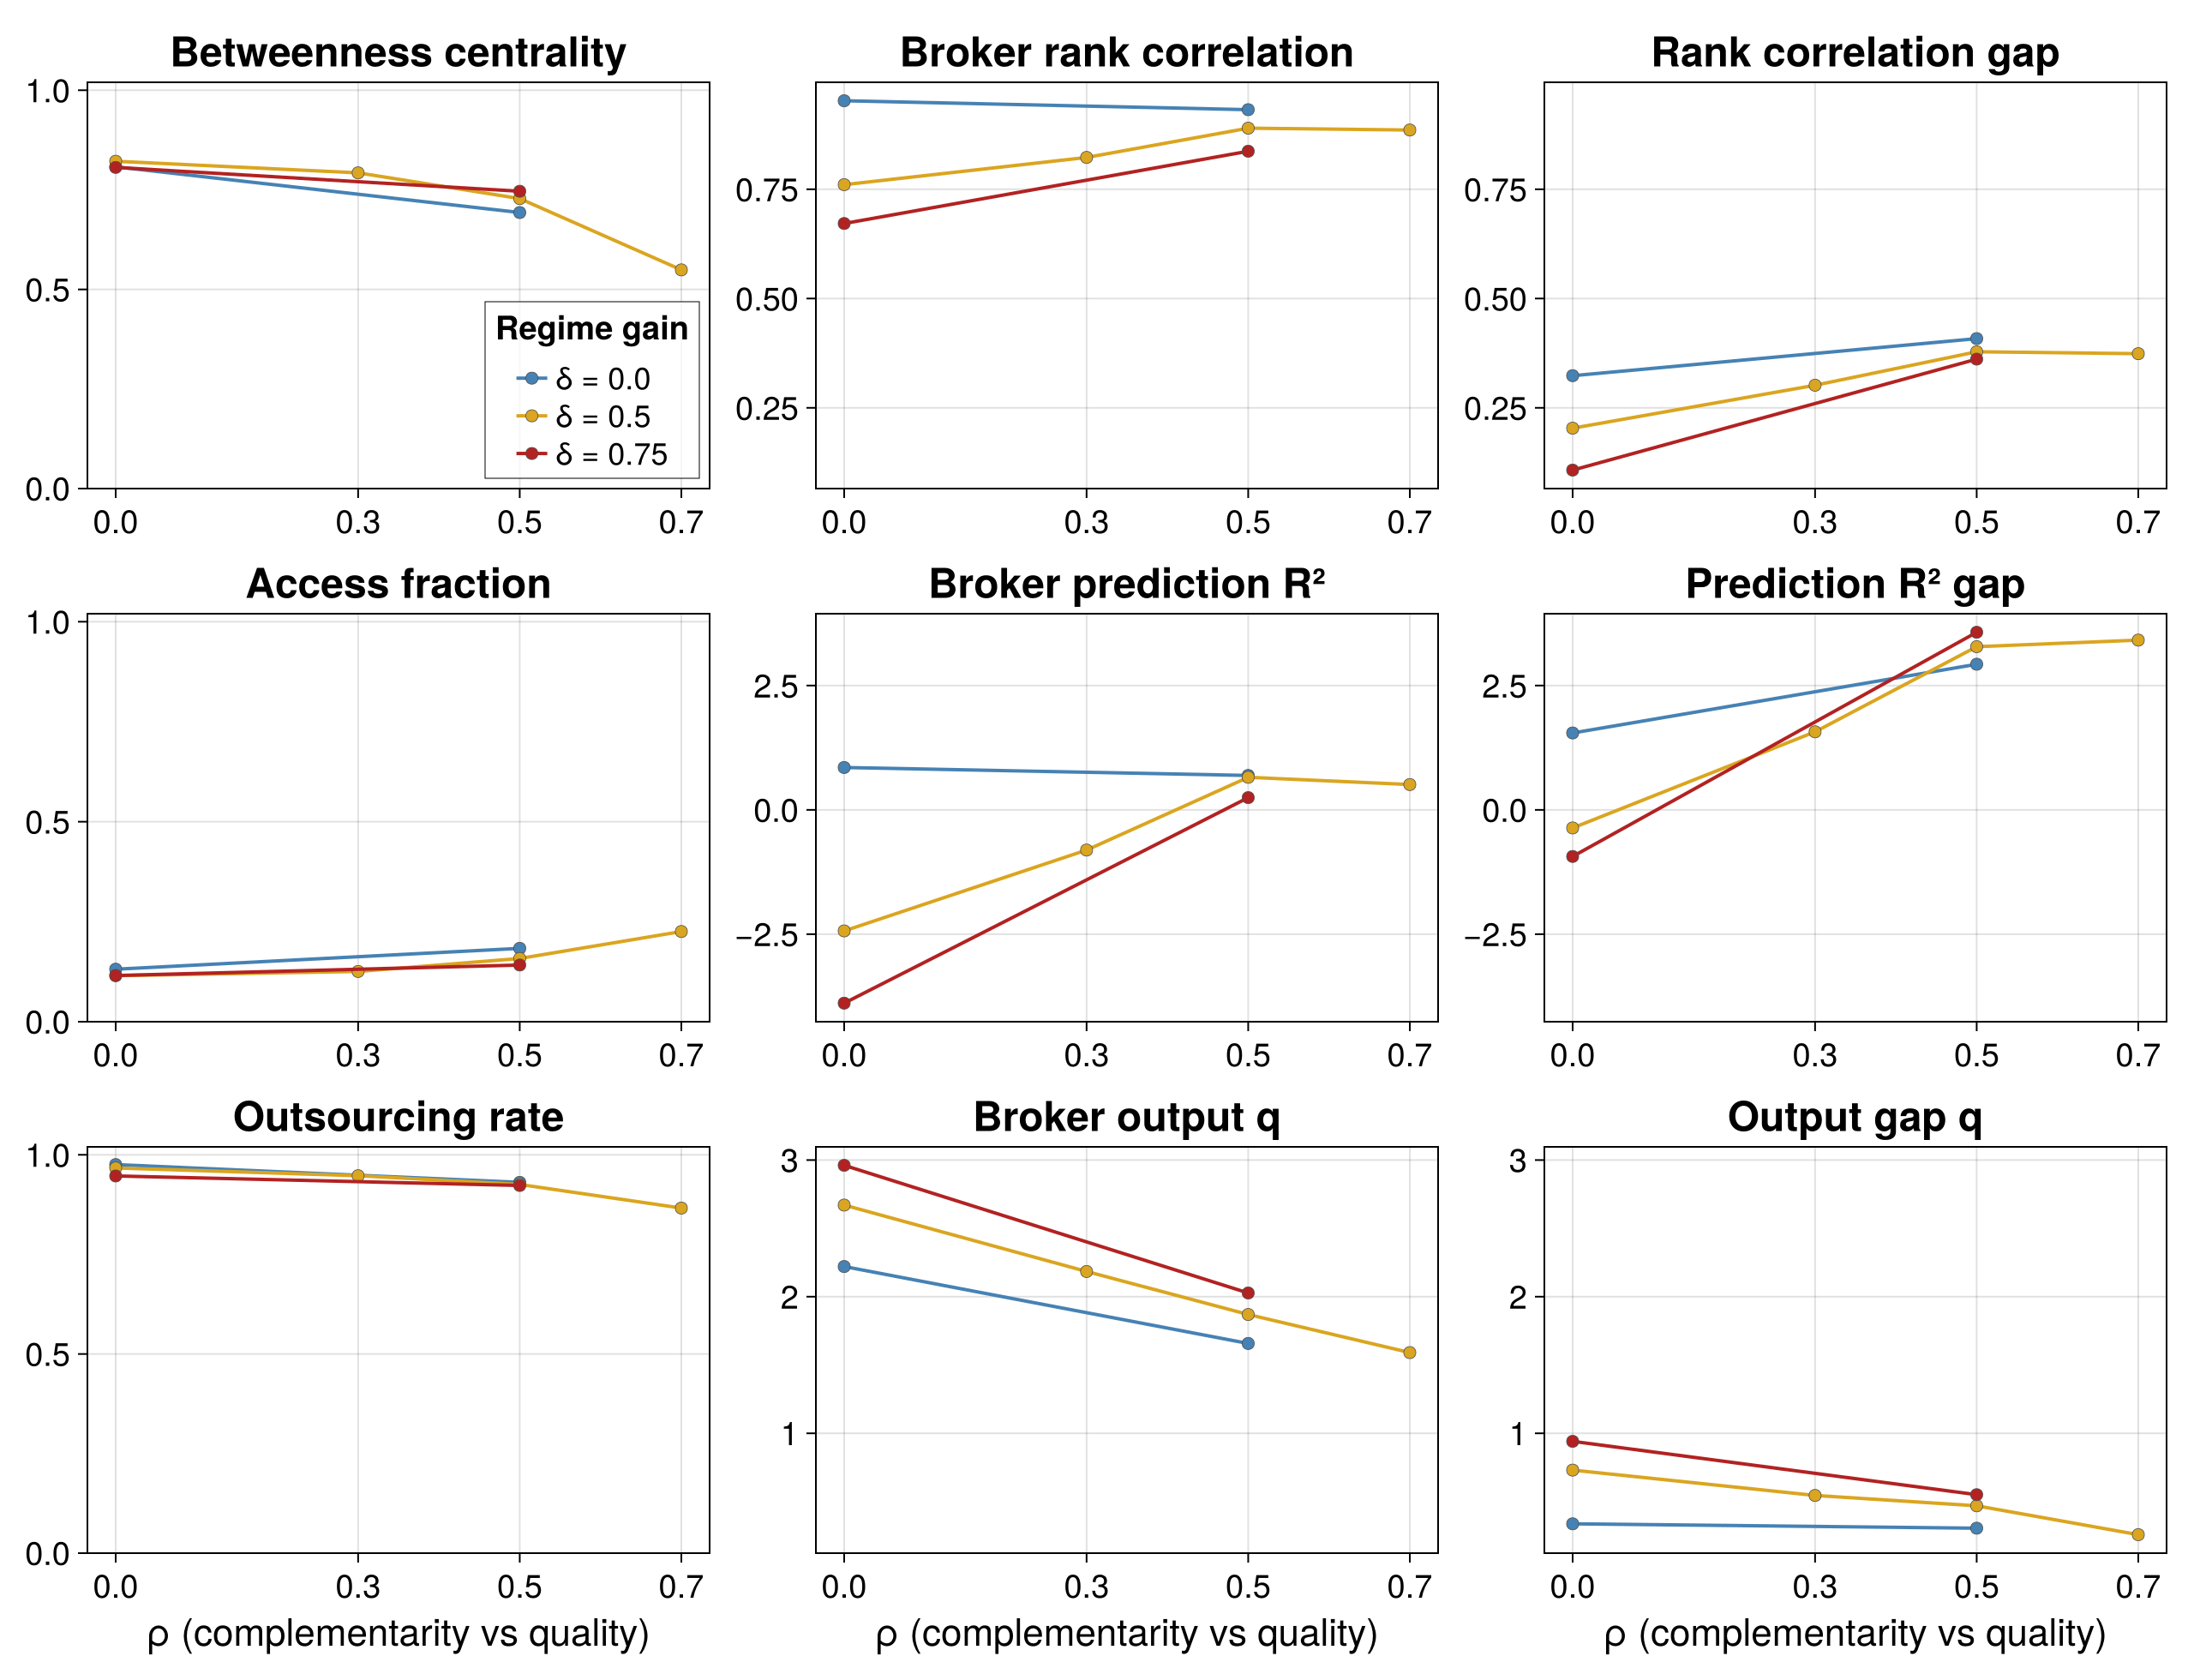
\includegraphics[width=\linewidth]{figs/fig3_grid_lines.png}
\caption{Late means of nine outcomes across the $\rho\times\delta$ grid (no
capture; $\rho=1$ omitted; one-at-a-time $\rho$ regimes refine the $\delta=0.5$
line), one line per gain $\delta$. The first column is on the unit scale; in
columns two and three, panels in the same row share a y-axis.}
\label{fig:grid}
\end{figure}

\subsection{Opportunity, behavior, and the production of structural advantage}

In almost all regimes, the broker's structural position strengthens over time and
the agent network thins. At the no-capture baseline, mean agent degree falls
(27.1 to 23.1, early to late means) and the
broker's betweenness centrality rises (0.60 to
0.73), and this co-movement holds in 86 of 91
no-capture regimes (Fig.~\ref{fig:position}). Turnover removes ties about as fast
as they appear, and the network does not densify: agent degree falls within the
run in 90 of 91 regimes. This raises a crucial question: why
is the structural advantage not self-liquidating, even at low turnover (at
$\eta=0.01$, betweenness still rises, from 0.45 to
0.62)?

The answer comes from the fact that structural position is endogenous, produced by
which agents form ties and which agents go to the broker. A brokered match adds a
new agent-to-agent tie, after which the broker no longer lies on the pair's
shortest path, only when the two were not already connected
(Appendix~A~\S5b,~\S8). Hence the broker's work densifies the network only when it
provides access, not when it provides assessment, and across regimes access is
rare and falling. The pure-quality regimes ($\rho=1$) come closest to escaping
this logic: agents there predict quality well from attributes and match well on
their own, outsourcing is somewhat lower (0.87 against
0.95 at $\rho=0$, late means), and brokered matches are twice as
often access (0.24 against 0.12). Yet these
regimes do not so much self-liquidate the broker's position as never let it
accumulate: the broker's centrality is far lower to begin with (a late mean of
0.13 across $\rho=1$ regimes, against 0.73 at
baseline) and stalls rather than rises, the access share still declines within
runs, and the network still thins in 13 of the 14 such
regimes; the five exceptions to the co-movement above are all of this type. Only
in the pure-quality regime with the highest reservation threshold ($f_r=1.2$) does
agent degree actually rise within the run. Identifying regimes in which brokered
access dominates and densification erodes the broker's position remains an open
question.

Across no-capture regimes, the broker's structural advantage, measured by
betweenness centrality, is negatively correlated with the access fraction
($-0.66$, late means): the broker is most central where it bridges
least. Bridging opportunity and bridging behavior thus move in opposite directions
across regimes, another counter-intuitive pattern in light of existing theory.
Clients value the broker's assessment services and outsource in large numbers, and
the broker's ties to its many clients are what make it central; its advantageous
position, however, is not accompanied by more access matches. This pooled
correlation is dominated by the $\rho$ axis: within single-parameter families it
changes sign (positive along the $\eta$ and $N$ sweeps, $+0.99$
and $+0.82$; negative along the $f_r$ and $\rho$ sweeps,
$-0.98$ and $-0.90$).

Because access is low throughout (a late mean of 0.16 across
no-capture regimes, declining within runs), the densifying effect is weak and the
broker's structural advantage persists. Where brokering is assessment rather than
access, self-liquidation of the structural advantage need not arise.

Realized output tracks betweenness centrality, not access fraction or prediction
quality: across no-capture regimes (late means), the output gap is positively
correlated with broker betweenness ($+0.82$) and negatively with the
access fraction ($-0.46$) and the broker's holdout rank correlation
($-0.66$) (Fig.~\ref{fig:advantage}). These correlations
describe co-variation across the design grid (91 regimes, five seeds each;
they characterize the grid, not a sampled population), and the matching problem
moves both sides of them. Complementarity-dominated regimes ($\rho=0$) are sparse
and brokered-assessment-heavy: agents hold fewer ties, outsource more of their
demand, and the broker is at once most central and most valuable, while providing
the least access (Table~\ref{tab:rhogroups}). Quality-dominated regimes ($\rho=1$)
sit at the other end of each of these measures, with the baseline level in
between. Structural opportunity thus accumulates exactly where the broker's
matches are worth the most; whether the position itself contributes to the
realized advantage is not identified by the grid, since the same parameter that
makes the broker central also makes its assessment matter.

\begin{table}[t]
\centering\small
\caption{Regime-group means at the three $\rho$ levels, no capture (late means).
Each group pools the 14 regimes of the $\rho$ family at that level:
the one-at-a-time $\rho$ regime and the $\rho$-paired grid cells. Output gap is
the realized value of broker-channel matches minus self-search matches.}
\label{tab:rhogroups}
\begin{tabular}{lccccc}
\toprule
 & Mean agent degree & Outsourcing rate & Broker betweenness & Access fraction & Output gap \\
\midrule
$\rho=0$   & 18.6  & 0.95  & 0.81  & 0.12  & $+0.71$ \\
$\rho=0.5$ & 23.2 & 0.91 & 0.72 & 0.16 & $+0.44$ \\
$\rho=1$   & 31.6  & 0.87  & 0.13  & 0.24  & $+0.10$ \\
\bottomrule
\end{tabular}
\end{table}

\begin{figure}[t]
\centering

\includegraphics[width=0.92\linewidth]{figs/fig4_advantage.png}
\caption{Rank-correlation gap (broker minus agent) and output gap (broker minus
self) against broker betweenness and access fraction; late means, one dot per
no-capture regime. Color gives $\rho$; marker size gives the effective rank
$r_{90}$.}
\label{fig:advantage}
\end{figure}

\subsection{Conditions and consequences of capture}

In the capture variant, the broker may stop working on behalf of a client and
instead buy that client's demand and place it as a principal (Appendix~A~\S9).
How much it does so varies with the features that shape its advantage, and with
the risk it must bear.

Capture by the broker is most extensive where matching is
complementarity-dominated: the captured share of outsourced demand (late means) is
0.97, 0.96, and 0.93 at $\rho=0$, $0.3$, and $0.5$, and
lower toward the quality end (0.77 and 0.76 at $\rho=0.7$ and
$1$). The sharpest control for capture rates is the reservation threshold $f_r$,
which sets the inventory risk the broker takes on (see model description): the
captured share is 1.00, 0.93, 0.78, and 0.20 at
$f_r=0.4$, $0.6$, $0.9$, and $1.2$ (Fig.~\ref{fig:capture}). Capture rates are
largely insensitive to problem difficulty (0.99 at $\delta=0$ against
0.96 at $\delta=0.75$) and to the pace of agent turnover (0.99,
0.93, 0.94 at $\eta=0.01$, $0.02$, $0.03$), and vary
non-monotonically with market size (0.80, 0.93, 0.83 at
$N=500$, $1{,}000$, $1{,}500$).

Capture is therefore most extensive where matching is relational and the risk of
acting as principal is smallest. The reservation threshold isolates the risk
channel cleanly: as $f_r$ rises, the captured share falls monotonically while the
broker's loss rate on captured positions mounts (0.06, 0.16,
0.35, 0.52 across the $f_r$ sweep, late means). Along $\rho$, by
contrast, the candidate sources of advantage co-vary: the regimes where the broker
captures most are also those where it is most central and its matches most
valuable, even though its ranking edge over the agents is there at its smallest
(Sec.~\ref{sec:matching-shapes}), so the design does not separate which of them
capture follows.

\begin{figure}[t]
\centering
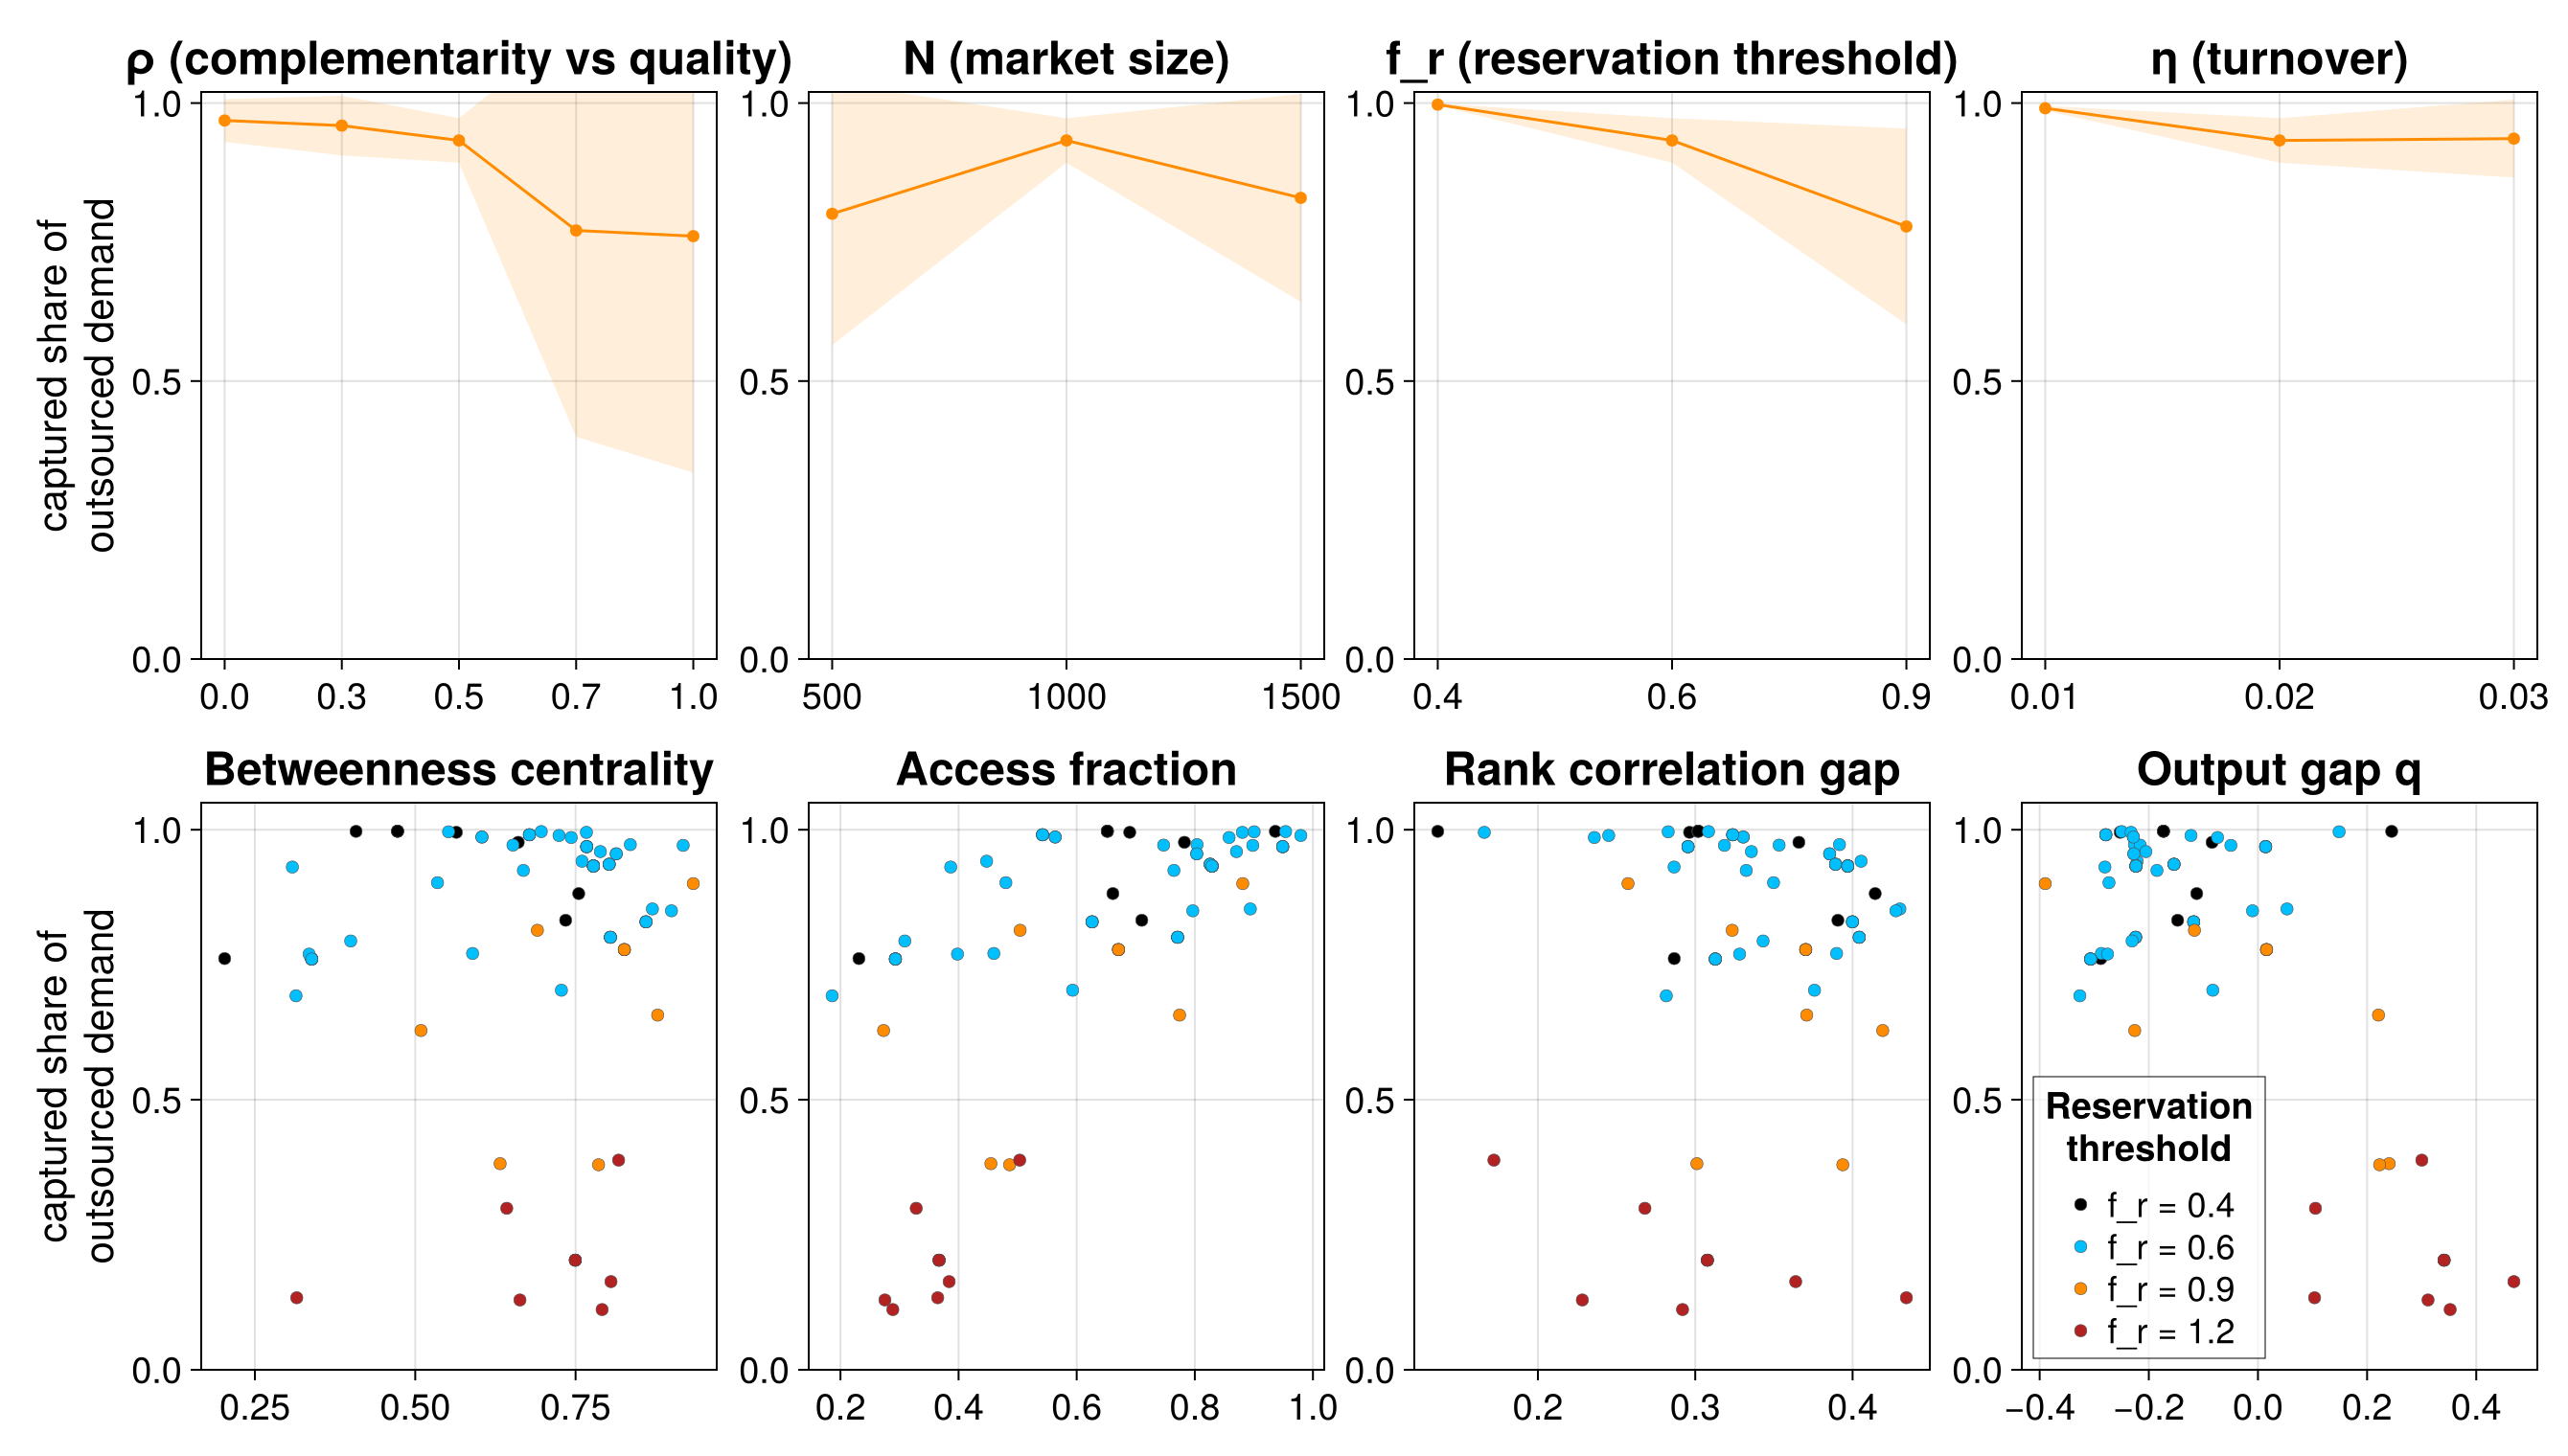
\includegraphics[width=\linewidth]{figs/fig5_capture.png}
\caption{Captured share of outsourced demand. Top row: late means (line) and
$\pm 1$ SD over seeds (band) along the $\rho$, $N$, $f_r$, and $\eta$ sweeps.
Bottom row: captured share against four late-mean outcomes, one dot per capture
regime (all 94), colored by $f_r$.}
\label{fig:capture}
\end{figure}

\begin{table}[t]
\centering\footnotesize
\setlength{\tabcolsep}{3pt}
\caption{The baseline regime pair (late means unless noted). Outsourcing: share of
match demand sent to the broker. Captured: captured share of outsourced demand.
Degree: mean agent degree. Matches: matches per agent per period. Betweenness:
broker betweenness. Access: access fraction. Satisfaction: mean satisfaction with
the broker channel, early to late mean. Agent holdout: principals' rank
correlation and $R^2$ on the random-partner holdout. Obs.: agent training
observations per period.}
\label{tab:baseline}
\begin{tabular}{lcccccccccc}
\toprule
 & Outsourcing & Captured & Degree & Matches & Betweenness & Access &
Satisfaction & \multicolumn{2}{c}{Agent holdout} & Obs. \\
\cmidrule(lr){9-10}
 & & & & & & & (early $\to$ late) & rank & $R^2$ & \\
\midrule
No capture & 0.93 & n/a & 23.1 & 4.9
 & 0.73 & 0.16
 & 1.65 $\to$ 1.77
 & 0.51 & $-2.63$ & 4,862 \\
Capture & 0.72 & 0.93 & 10.5 & 4.7
 & 0.78 & 0.83
 & 1.36 $\to$ 1.25
 & 0.51 & $-1.15$ & 1,441 \\
\bottomrule
\end{tabular}
\end{table}

Capture reorganizes the market (Table~\ref{tab:baseline}; Fig.~\ref{fig:dynamics}).
Because a principal
placement connects the broker to each side but creates no tie between the two
clients, the agent network thins out: at the baseline pair, mean agent degree
under capture is about half its no-capture level, while matches per agent are
essentially unchanged and flat within runs: what changes is who gets connected,
not how much matching occurs. The broker's own betweenness is slightly higher.
The access fraction reverses, high and rising within runs under capture
(from 0.60 early to 0.83 late at the capture
baseline, against 0.16 without capture; it rises within the run
in 72 of 94 capture regimes), because in a
thinned network the broker is increasingly the only path between agents. The
self-liquidating densification of ordinary brokerage, in which each match erodes
the gaps the broker bridges, is suspended.

\begin{figure}[t]
\centering
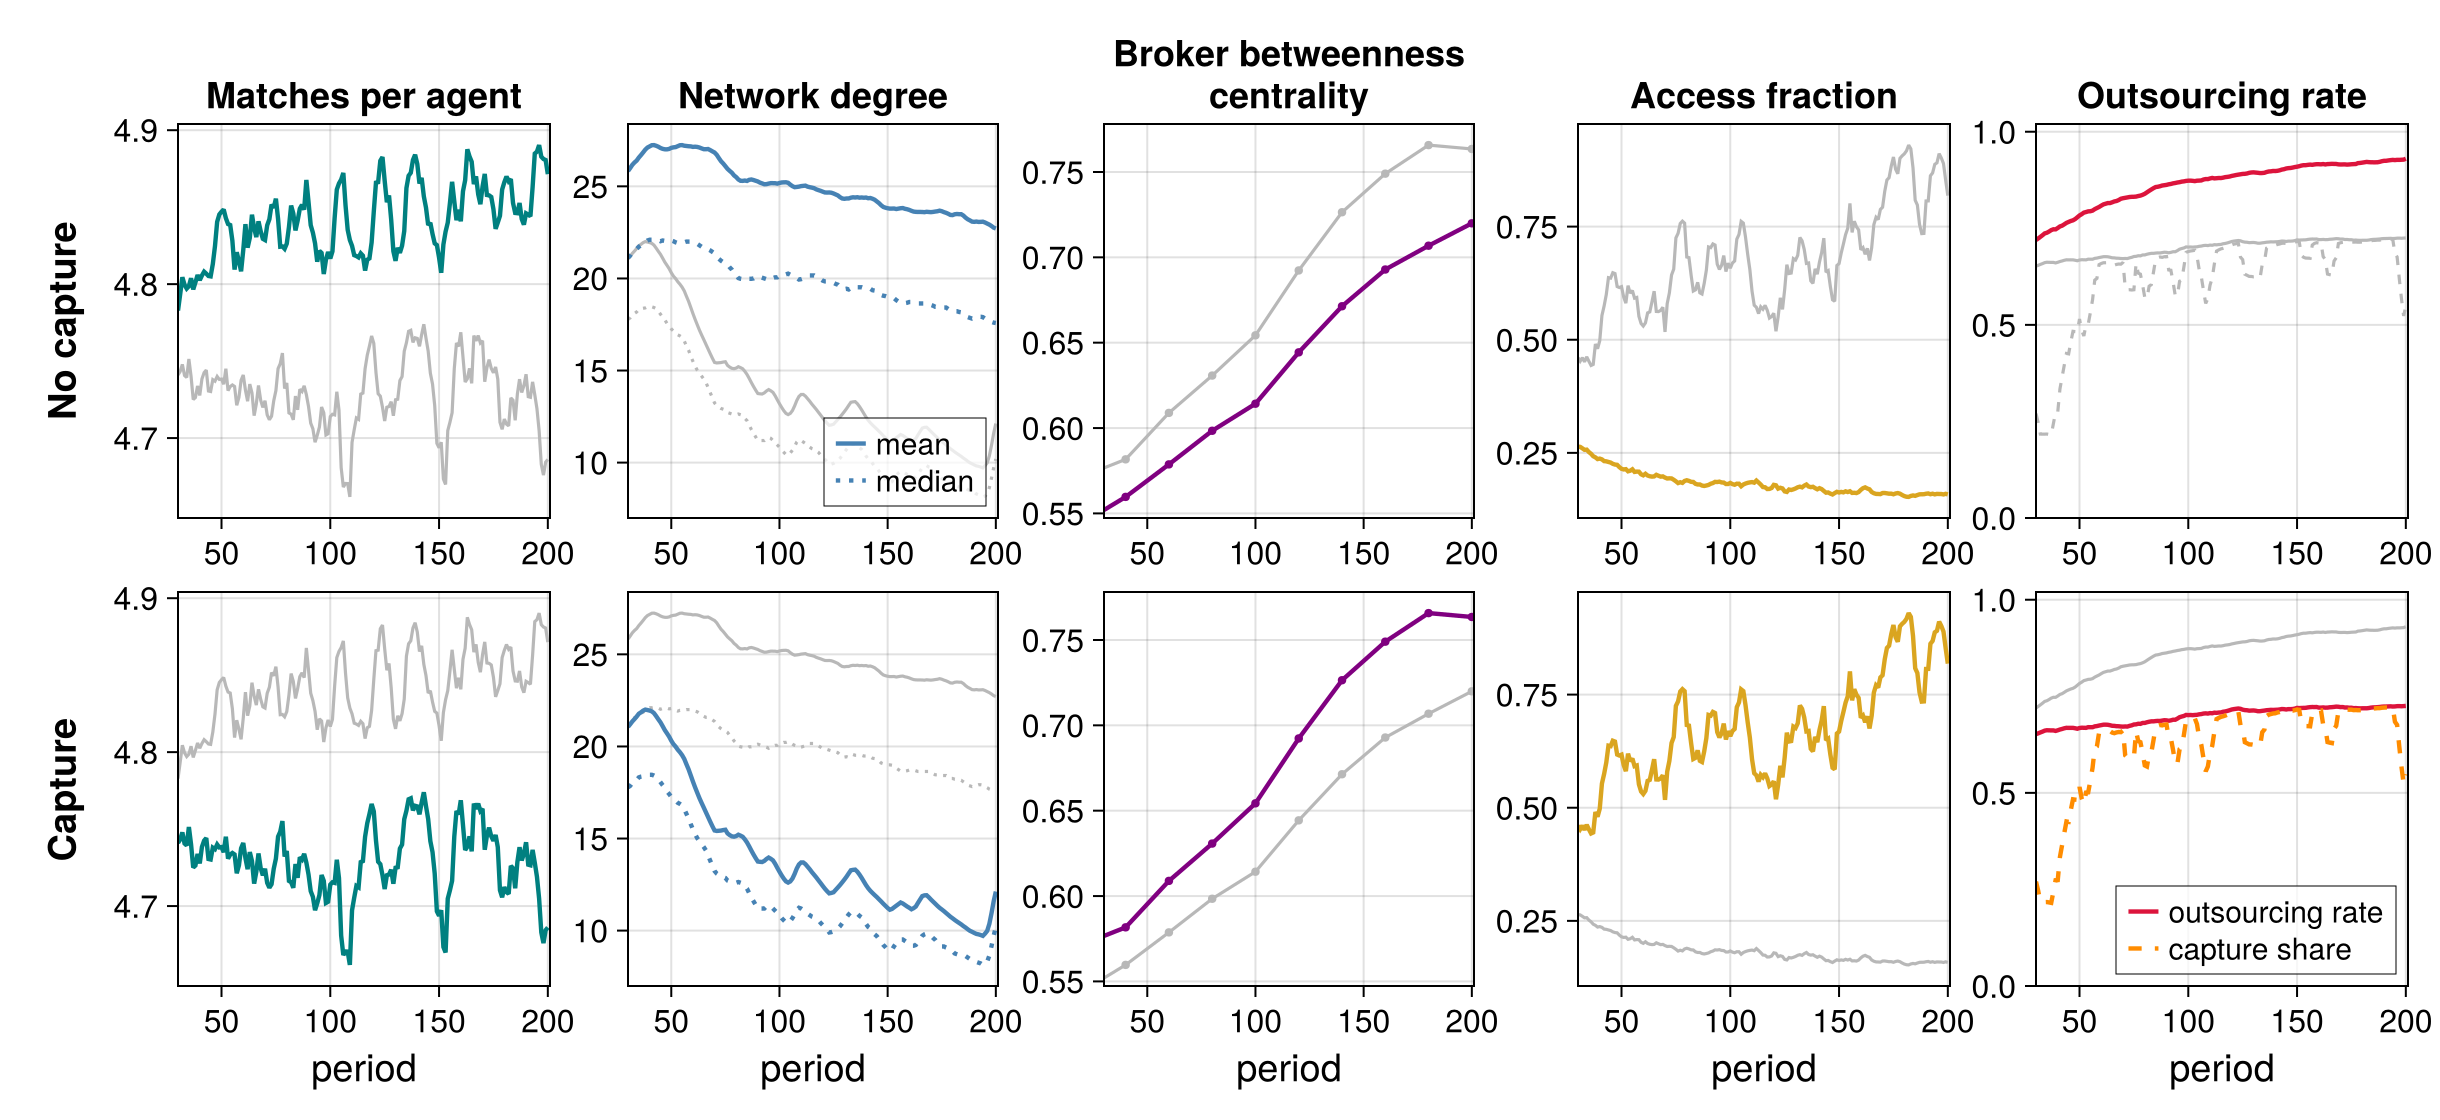
\includegraphics[width=\linewidth]{figs/fig6_dynamics.png}
\caption{Baseline dynamics over time without capture (top row) and with capture
(bottom row): matches per agent, agent degree (mean and median), broker
betweenness, access fraction, and outsourcing rate. Lines are 5-observation
rolling ensemble means; betweenness is rolled over its 20-period measurements. In
each panel, pale gray reproduces the corresponding series of the other row. The
capture row's last panel adds the captured share of total demand (dashed). Panels
in the same column share y-ranges; axes start at $t=30$.}
\label{fig:dynamics}
\end{figure}

Outsourcing is also lower under capture (late means of 0.70
against 0.90 across regimes), because of the interaction between
the pricing and decision rules. A captured client is paid its own historical
average realized value (Appendix~A~\S9): at the capture baseline (late means),
captured clients are paid about 1.29 per slot, while standard
brokered matches realize 1.46 and the positions the broker
keeps realize 1.69. Since standard brokered matches realize
above-average value, clients tend to be less satisfied with being bought out by
the broker than with concluding a brokered match: in the capture baseline, mean
satisfaction with the broker channel falls from the early to the late window,
while in the no-capture baseline it rises (Table~\ref{tab:baseline}), returning
some demand to self-search.

Captured transactions freeze the clients out of forming new ties, and this lock-in
produces the thinning network described above. By the same token, capture removes
learning opportunities: principal placements are recorded only in the broker's
history, so agents learn from fewer matches under capture than without it
(2,102 against 4,810 observations per period, late
means across the 91 paired regimes; 55\% of matches
under capture write nothing to the agents).

Yet, on the measures of prediction performance on a holdout set, the agents
perform no worse than without capture. At the baseline pair, their ranking is
essentially unchanged and their level calibration is better
(Table~\ref{tab:baseline}); the pattern holds across the 91 paired
regimes (rank 0.54 against 0.51; $R^2$
of $-1.41$ against $-2.73$). Indeed, agents'
holdout performance deteriorates within runs in both variants even as their
histories grow (across the no-capture regimes, rank 0.56
to 0.51 and $R^2$ $-1.63$ to
$-2.73$ from the early to the late window; milder under capture).
One reading, which is not tested here, is that without capture, when outsourcing
is high, the clients' out-of-sample weakness comes mainly from learning on a
selected sample, the broker's top-scored pairings; capture reduces the outsourcing
rate, makes the sample clients observe less selected, and selection deepens as
runs progress. A fuller account of client learning, with and without capture, is
deferred to future work.
